\section{The Simulation}\label{sec:the-simulation}

In this section, we discuss the main elements of the simulation.
To fully understand the concepts that are discussed here, such as nodes and programs, please refer to the~\href{https://alchemistsimulator.github.io/}{Alchemist documentation}.

\subsection{Map Environment}\label{subsec:map-environment}
The simulation concerns an existing geographical location, that is the amusement park of~\href{https://www.mirabilandia.it/}{\textit{Mirabilandia}}.
For this reason, the environment of the simulation must be a map featuring existing paths in the real world.
To achieve this, \textit{Alchemist} allows using maps provided by \href{https://www.openstreetmap.org/}{\textit{OpenStreetMap}}, the free wiki world map. \textit{OpenStreetMap} provides navigation capabilities on the whole planet;
such data, weighs about 50GB, thus it is recommended to use an extract with the data relative to the interested area.
One great way to obtain an extract is through~\href{https://extract.bbbike.org/}{\textit{BBBike}}~\cite{Pianini_2013}.

Once extracted the map in the \texttt{.pbf} format, it is possible to build the simulation environment through the~\href{https://alchemistsimulator.github.io/reference/kdoc/alchemist/it.unibo.alchemist.model.implementations.environments/-o-s-m-environment/}{\texttt{OSMEnvironment}}, as shown in the following listing (\ref{lst:osm}).

\begin{lstlisting}[language=yaml, label={lst:osm}, caption=Building an \textit{OpenStreetMap} environment.]
# Use an OpenStreetMap Environment,
# deploying nodes only on streets.
environment:
  type: OSMEnvironment
  parameters: [mirabilandia.osm.pbf, true]
\end{lstlisting}


\noindent
The constructor of the environment accepts two parameters:
\begin{itemize}
    \item \texttt{file: String}, the path to the file containing the exported map;
    \item \texttt{onlyOnStreets: Boolean}, a boolean value allowing to deploy nodes only on the streets.
\end{itemize}

\subsection{Deployed Nodes}\label{subsec:deployed-nodes}
After setting the environment, it is essential to deploy \textbf{nodes} on the map.
In the current simulation, the elements that are represented by nodes are:
\begin{itemize}
    \item \textbf{Visitors}, as single individuals or groups;
    the key point here is that a node should correspond to one or more people using a single wearable device that tracks and guides its owner.
    \item \textbf{Attractions}, that can be of different types, such as rides, water slides, restaurants, etc.; they are considered \textit{rendezvous} points for visitors and are made of several sensors that allow keeping track of various information, such as the number of people waiting in a queue.
\end{itemize}

\noindent
In order to deploy nodes on the map it is mandatory to declare them under the \texttt{deployments} section, as shown in the following listing.

\begin{lstlisting}[language=yaml, label={lst:deployment}, caption=Deploying 1 attraction and 100 visitors inside the \texttt{bounds} polygon.]
# Define visitors
_visitors: &visitors
  - type: Polygon
    parameters: [ 100, *bounds ]
    contents:
      - { molecule: visitor, concentration: true }

# Define attractions
_attractions: &attractions
  - type: Point
    parameters: [44.33589, 12.26293]
    contents:
      - { molecule: attraction, concentration: true }
      - { molecule: attractionType, concentration: "\"restaurant\"" }
      - { molecule: capacity, concentration: 10 }
      - { molecule: name, concentration: "\"McDonald's\"" }

# Deploy nodes
deployments:
  - *attractions
  - *visitors
\end{lstlisting}


\noindent
Moreover, it is necessary to explicit which \textbf{linking rule} will be used to connect nodes with each other.
As for the current simulation, the proper way to connect nodes cannot be based on a geometric rule (for instance, connecting nodes within a certain distance).
Instead, it is appropriate to consider attractions as \textbf{access points} for the visitors' devices.
Even with the~\href{https://alchemistsimulator.github.io/reference/kdoc/alchemist/it.unibo.alchemist.model.implementations.linkingrules/-connect-to-access-point/index.html}{\texttt{ConnectToAccessPoint}} linking rule every node on the map will be connected with the rest of the network as the attractions are distributed throughout the map, and, working as access points, they can cover it without leaving connectionless areas.

\begin{lstlisting}[language=yaml, label={lst:linking}, caption=Defining the linking rule: only nodes with the molecule \texttt{attraction} will connect to other nodes within a radius of 100 meters.]
# The network model used allows to choose the nodes that have the
# "attraction" molecule in order to simulate an access point behaviour
network-model:
  type: ConnectToAccessPoint
  parameters: [100.0, "attraction"]
\end{lstlisting}


\subsection{Programmed Behaviours}
With both the environment and the nodes correctly set, the next step consists in programming their behaviours.
Each and every node needs to implement a proper behaviour depending on its type.
In particular, visitors and attractions will have different behaviours: for instance, visitors should move on the map in order to get to attractions, while the latter should stay still and satisfy enqueued visitors.
The behaviours are written using the \textit{Protelis} aggregate language.
Although, performing local computations using a programming language designed for the aggregate paradigm is probably not the best choice.
So, it is appropriate to implement local computations with a different language.
Therefore, for this simulation, also \textit{Kotlin} was used.
The following sections describe the behaviours implemented by visitors and attractions.

\subsubsection{Attractions' Positions}
In order to make each visitor node aware of the positions of all the attractions in the map, it is necessary to implement a behaviour that spreads the desired information.
To do so, it is useful to use \textit{aggregate programming}.
Specifically, \textit{Alchemist} allows inserting an external program into a node, as shown in the following listing.

\begin{lstlisting}[language=yaml, label={lst:positions}, caption=Assign the \texttt{org:protelis:microcity:positions} behaviour to 100 visitors and 2 attractions.]
# Define the broadcast message from attractions to visitors
# to spread their positions
_positions: &positions
  - time-distribution: 1
    program: org:protelis:microcity:positions
  - program: send

# Define visitors
_visitors: &visitors
  - type: Polygon
    parameters: [ 100, *bounds ]
    programs: *positions
    contents:
      - { molecule: visitor, concentration: true }

# Define attractions
_attractions: &attractions
  - type: Point
    parameters: [44.33747, 12.26208]
    programs: *positions
    contents:
      - { molecule: attraction, concentration: true }
  - type: Point
    parameters: [ 44.33815, 12.2633 ]
    programs: *positions
    contents:
      - { molecule: attraction, concentration: true }
\end{lstlisting}


On the other hand, the definition of the aggregate program should describe how the desired information is spread as a field.
In particular, each node should gather the field from its neighbours and merge the received values.
The listing~\ref{lst:protelis-positions} shows how it is possible to implement this behaviour in \textit{Protelis}.

\begin{lstlisting}[label={lst:protelis-positions}, caption=Sharing the coordinates of each attraction to all the nodes that implement this behaviour.]
module org:protelis:microcity:positions

import microcity.Positions.attractionPositions
import microcity.Positions.attractionUnion

share (field <- attractionPositions()) {
    foldHoodPlusSelf(field, { a, b -> attractionUnion(a, b) })
}
\end{lstlisting}


The \texttt{attractionPositions} function simply builds a list with the node's position if it presents an ``attraction" molecule, otherwise an empty list.
In this way, the field is composed by lists of positions containing only attractions' coordinates.
The \texttt{attractionUnion} function just unifies the received lists into a single one.

\subsubsection{Queues \& Satisfaction}
Similarly to positions, it is necessary to keep track of the queues that form nearby attractions and broadcast them to visitors.
The queue formed nearby an attraction is determined by the sequence of visitors that have the same coordinates as the attraction.
Though, it is important that the visitors waiting in the queue are not satisfied.
In fact, a visitor's satisfaction is a condition that only occurs after it has benefited from an attraction.
When satisfied, the visitor is then ready to choose the next destination, and, once the next attraction is decided, it can switch back to unsatisfied.
These behaviours can be split into 3 different \textit{Protelis} programs:
\begin{itemize}
  \item \textbf{\texttt{queue}}: given an attraction, determine the list of visitors that are enqueued to it.
  \item \textbf{\texttt{queues}}: broadcast the queues of every attraction to every visitor.
  \item \textbf{\texttt{satisfaction}}: given an attraction, satisfy the first $N$ visitors in its queue, where $N$ represents the attraction's capacity.
\end{itemize}

\noindent
All these behaviours are programmed by both attractions and visitors.
The \texttt{satisfaction} program has a lower time distribution, as it is assumed that it takes a while for an attraction to satisfy visitors.

\subsubsection{Movement}\label{subsubsec:movement}
Movement is a feature only owned by visitors.
It is implemented as a \href{https://alchemistsimulator.github.io/reference/kdoc/alchemist/it.unibo.alchemist.model.implementations.actions/-target-map-walker/index.html}{\texttt{TargetMapWalker}}: this action needs a ``tracking" molecule inside the implementing node that has a destination's coordinates as its concentration.
Moreover, the latter allows nodes to move only on maps' streets, adapting to the provided~\href{https://alchemistsimulator.github.io/reference/kdoc/alchemist/it.unibo.alchemist.model.implementations.environments/-o-s-m-environment/}{\texttt{OSMEnvironment}}.

As discussed in the section~\ref{sec:the-case-study}, in order to decide its next destination, a visitor can adopt one of these two policies: \textbf{Random Redirection} or \textbf{Recommended Redirection}.
In order to achieve this, visitors also own a program that establishes the next destination with one of the two policies and inserts its coordinates in a molecule.
The listing~\ref{code:movement} shows how the \texttt{TargetMapWalker} behaviour and the \texttt{destination} behaviour are assigned to the visitor nodes.

\begin{lstlisting}[language=yaml, label=code:movement, caption=Define the movement behaviour for visitors.]
# Define the movement law with a Walker that moves only on streets towards
# a GeoPosition indicated by the concentration of the tracking molecule
_move: &move
  - time-distribution: 1
    type: Event
    actions:
      - type: TargetMapWalker
        parameters: [org:protelis:microcity:destination, 1.0]

# Define the rule that establishes how visitors choose the
# next destination
_destination: &destination
  - time-distribution: 1
    program: org:protelis:microcity:destination
  - program: send
\end{lstlisting}


In order to choose the next destination for a visitor, a \textit{Protelis} program will call a function \texttt{getNext} that will return the coordinates of the next attraction.
It is possible to define a custom policy just by implementing the interface \texttt{NextPolicy}, and therefore defining the method \texttt{getNext}.
For the sake of the current simulations, the following policies were provided:
\begin{itemize}
    \item \texttt{RandomPolicy}: performs a \textit{random redirection} by choosing one of the attractions inside the park randomly.
    \item \texttt{ShortestQueuePolicy}: performs a \textit{recommended redirection} by choosing the attraction with the shortest queue inside the whole park.
    \item \texttt{ShortestQueueInRangePolicy}: performs a \textit{recommended redirection} by choosing the attraction with the shortest queue within a given range with regard to the visitor.
\end{itemize}

\subsection{Data Extraction \& Evaluation}\label{subsec:data-extraction}
The whole point of the simulations consists in determining whether a \textit{situated recommendation system} may help reduce the waiting time for visitors inside the park.
In order to evaluate that, it is necessary to extract data from the simulation.
In particular, the data we extracted and analyzed concerns the amount of time spent in a queue and the number of attractions that every visitor has benefited from.
Data extraction is achieved thanks to the implementation of an~\href{https://alchemistsimulator.github.io/reference/kdoc/alchemist/it.unibo.alchemist.loader.export/-extractor/index.html}{\texttt{Extractor}} that allows controlling and exploring the environment at each simulation step.
Thanks to that, it was possible to address the waiting time of a visitor to the amount of steps it spends in a queue.
On the other hand, counting the amount of times that a visitor has been satisfied by an attraction was possible thanks to a specific molecule \texttt{satisfactions}.
These two types of data, on average, considering both the \textit{random redirection} and the \textit{recommended redirection} systems, consent to state whether visitors benefit from more attractions and wait less time in queues or not;
thus, they are considered to be a reasonable way to evaluate the \textit{situated recommendation system}.

For the evaluation, the right way to obtain reliable data is to launch every simulation multiple times and finally consider the average values of such data.
The following evaluations are based on the data obtained from 10 simulation runs for each redirection policy described in the section~\ref{subsubsec:movement}.

\begin{figure}[H]
    \centering
    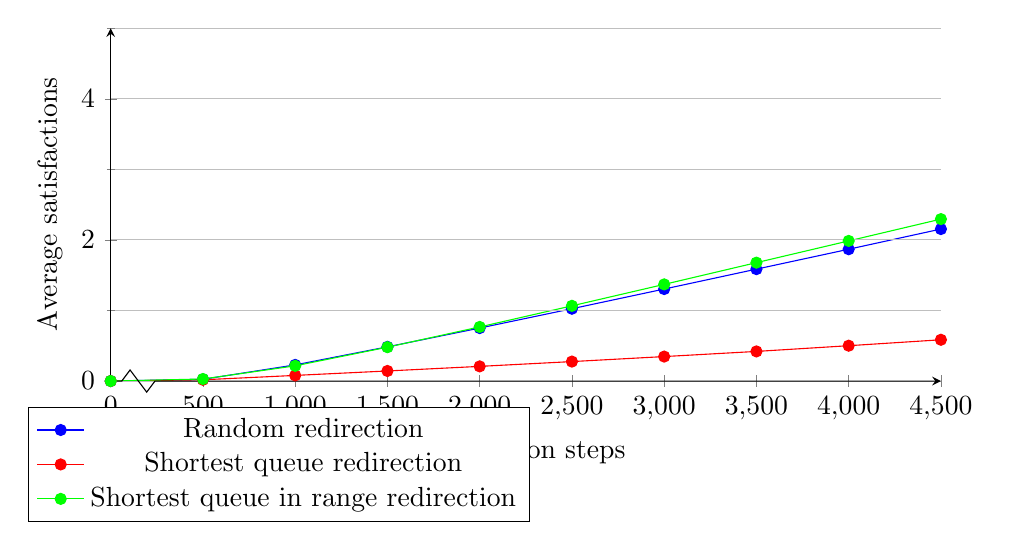
\begin{tikzpicture}
        \begin{axis}[
            xmin=0, xmax=4500,
            ymin=0, ymax=5,
            xtick={0, 500, ..., 4500},
            minor ytick={0,1,...,5},
            axis x line=bottom,
            axis y line=left,
            axis x discontinuity=crunch,
            ymajorgrids=true,
            yminorgrids=true,
            xlabel={Simulation steps}, ylabel={Average satisfactions}, title={},
            axis on top=true, clip=false,  width=\textwidth, height=.5\textwidth,
            legend style={
                at={(0,0)},
                anchor=south west,
                at={(axis description cs:-0.1, -0.4)}
            }
        ]
            \addplot [mark=*, color=blue] coordinates {
                (0, 0.0)
                (500, 0.025)
                (1000, 0.229)
                (1500, 0.485)
                (2000, 0.751)
                (2500, 1.025)
                (3000, 1.304)
                (3500, 1.586)
                (4000, 1.868)
                (4500, 2.154)
            };
            \addplot [mark=*, color=red] coordinates {
                (0, 0.0)
                (500, 0.018)
                (1000, 0.080)
                (1500, 0.143)
                (2000, 0.208)
                (2500, 0.276)
                (3000, 0.347)
                (3500, 0.420)
                (4000, 0.501)
                (4500, 0.585)
            };
            \addplot [mark=*, color=green] coordinates {
                (0, 0.0)
                (500, 0.029)
                (1000, 0.216)
                (1500, 0.480)
                (2000, 0.767)
                (2500, 1.066)
                (3000, 1.370)
                (3500, 1.678)
                (4000, 1.986)
                (4500, 2.295)
            };
            \legend{Random redirection, Shortest queue redirection, Shortest queue in range redirection}
        \end{axis}
    \end{tikzpicture}
    \caption{Average satisfactions for the three different redirection policies.}
    \label{plot:mean-satisfaction}
\end{figure}

As shown in the plot~\ref{plot:mean-satisfaction}, the number of satisfactions increases with the simulation steps.
The \textit{shortest queue redirection} is clearly the worst case, as visitors could cross the entire map in order to reach the attraction with the shortest queue.
Instead, \textit{shortest queue in range redirection} ensures that the next attraction will be within a certain range.
In this way visitors will walk less in order to reach attractions.
In fact, this policy brings on a higher number of satisfactions, even compared to the \textit{random redirection}.

\begin{figure}[H]
    \centering
    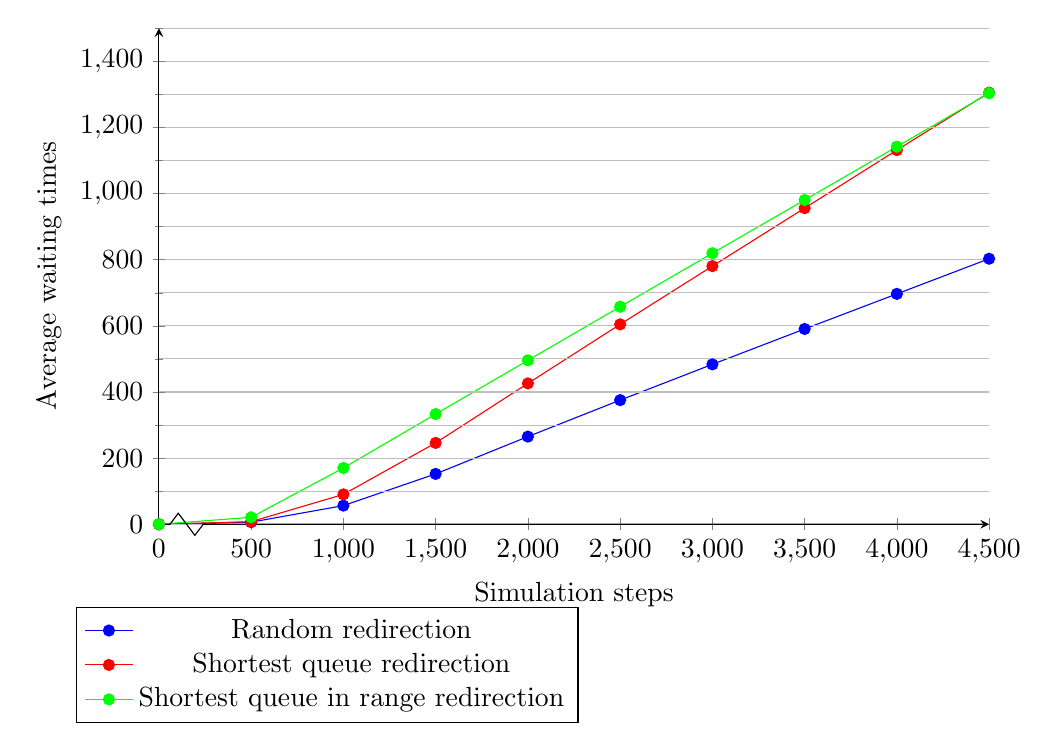
\begin{tikzpicture}
        \begin{axis}[
        xmin=0, xmax=4500,
        ymin=0, ymax=1500,
        xtick={0, 500, ..., 4500},
        minor ytick={0,100,...,1500},
        axis x line=bottom,
        axis y line=left,
        axis x discontinuity=crunch,
        ymajorgrids=true,
        yminorgrids=true,
        xlabel={Simulation steps}, ylabel={Average waiting times}, title={},
        axis on top=true, clip=false,  width=\textwidth, height=.65\textwidth,
        legend style={
            at={(0,0)},
            anchor=south west,
            at={(axis description cs:-0.1, -0.4)}
        }
        ]
        \addplot [mark=*, color=blue] coordinates {
            (0, 0.0)
            (500, 6.428)
            (1000, 56.439)
            (1500, 152.321)
            (2000, 265.101)
            (2500, 375.396)
            (3000, 483.579)
            (3500, 590.562)
            (4000, 696.678)
            (4500, 802.990)
        };
        \addplot [mark=*, color=red] coordinates {
            (0, 0.0)
            (500, 7.937)
            (1000, 90.407)
            (1500, 246.016)
            (2000, 425.997)
            (2500, 604.573)
            (3000, 780.633)
            (3500, 955.988)
            (4000, 1131.490)
            (4500, 1305.333)
        };
        \addplot [mark=*, color=green] coordinates {
            (0, 0.0)
            (500, 21.161)
            (1000, 170.291)
            (1500, 333.227)
            (2000, 495.653)
            (2500, 657.848)
            (3000, 819.695)
            (3500, 980.613)
            (4000, 1141.952)
            (4500, 1303.554)
        };
        \legend{Random redirection, Shortest queue redirection, Shortest queue in range redirection}
        \end{axis}
    \end{tikzpicture}
    \caption{Average waiting times for the three different redirection policies.}
    \label{plot:mean-waiting-times}
\end{figure}

As shown in the plot~\ref{plot:mean-waiting-times}, the waiting times increase with the simulation steps.
Paradoxically, the best case here is still the \textit{random redirection}.
This is probably due to the fact that, specially at first, visitors are walking to reach their first destinations.
In fact, the growth is slower at the beginning, but it increases after the first 1000 steps.
Indeed, comparing the two recommendation-based policies the best one remains the \textit{shortest queue in range redirection}.

However, increasing waiting times also mean that visitors spend more time in queues and less time walking in order to reach attractions.
Keeping in mind that the number of satisfaction is higher for this policy, this can be considered as a positive factor, since this result perfectly fits with the policy's aim.
So, the correct trend to evaluate is the waiting time per attraction, which is displayed in the plot~\ref{plot:waiting-time-per-attraction}.

\begin{figure}[H]
    \centering
    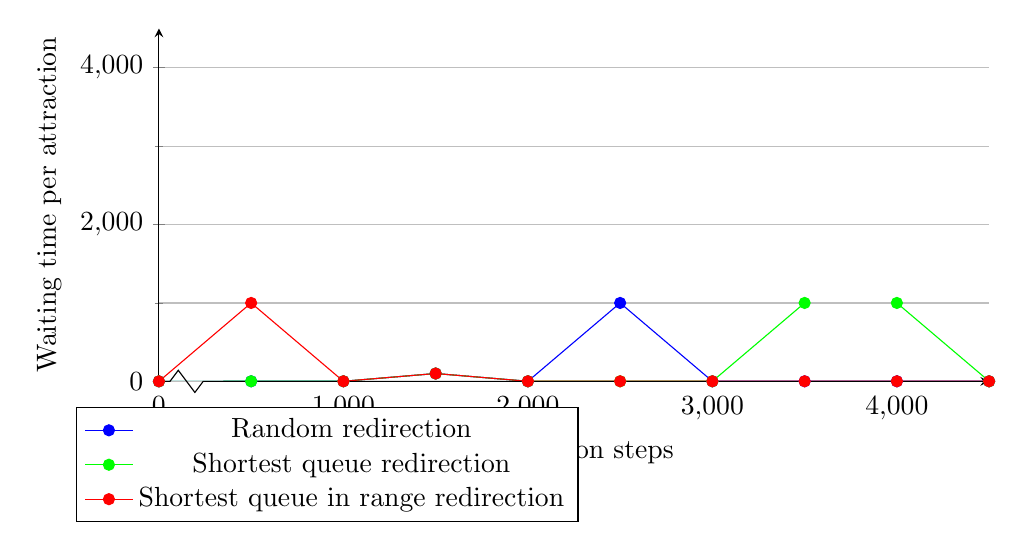
\begin{tikzpicture}
        \begin{axis}[
        xmin=0, xmax=4500,
        ymin=0, ymax=4500,
        xtick={0, 1000, ..., 4500},
        minor ytick={0,1000,...,4500},
        axis x line=bottom,
        axis y line=left,
        axis x discontinuity=crunch,
        ymajorgrids=true,
        yminorgrids=true,
        xlabel={Simulation steps}, ylabel={Waiting time per attraction}, title={},
        axis on top=true, clip=false,  width=\textwidth, height=.5\textwidth,
        legend style={
            at={(0,0)},
            anchor=south west,
            at={(axis description cs:-0.1, -0.4)}
        }
        ]
        \addplot [mark=*, color=blue] coordinates {
            (0, 0.0)
            (500, 1.0)
            (1000, 1.0)
            (1500, 100.0)
            (2000, 1.0)
            (2500, 1000.0)
            (3000, 1.0)
            (3500, 1.0)
            (4000, 1.0)
            (4500, 1.0)
        };
        \addplot [mark=*, color=green] coordinates {
            (0, 0.0)
            (500, 1.0)
            (1000, 1.0)
            (1500, 100.0)
            (2000, 1.0)
            (2500, 1.0)
            (3000, 1.0)
            (3500, 1000.0)
            (4000, 1000.0)
            (4500, 1.0)
        };
        \addplot [mark=*, color=red] coordinates {
            (0, 0.0)
            (500, 1000.0)
            (1000, 1.0)
            (1500, 100.0)
            (2000, 1.0)
            (2500, 1.0)
            (3000, 1.0)
            (3500, 1.0)
            (4000, 1.0)
            (4500, 1.0)
        };
        \legend{Random redirection, Shortest queue redirection, Shortest queue in range redirection}
        \end{axis}
    \end{tikzpicture}
    \caption{Waiting time per attraction for the three different redirection policies.}
    \label{plot:waiting-time-per-attraction}
\end{figure}
